% Options for packages loaded elsewhere
\PassOptionsToPackage{unicode}{hyperref}
\PassOptionsToPackage{hyphens}{url}
%
\documentclass[
  english,
  man]{apa6}
\title{DateLife: leveraging databases and analytical tools to reveal the dated Tree of Life}
\author{Luna L. Sánchez Reyes\textsuperscript{1,2}, Emily Jane McTavish\textsuperscript{1}, \& Brian O'Meara\textsuperscript{2}}
\date{}

\usepackage{amsmath,amssymb}
\usepackage{lmodern}
\usepackage{iftex}
\ifPDFTeX
  \usepackage[T1]{fontenc}
  \usepackage[utf8]{inputenc}
  \usepackage{textcomp} % provide euro and other symbols
\else % if luatex or xetex
  \usepackage{unicode-math}
  \defaultfontfeatures{Scale=MatchLowercase}
  \defaultfontfeatures[\rmfamily]{Ligatures=TeX,Scale=1}
\fi
% Use upquote if available, for straight quotes in verbatim environments
\IfFileExists{upquote.sty}{\usepackage{upquote}}{}
\IfFileExists{microtype.sty}{% use microtype if available
  \usepackage[]{microtype}
  \UseMicrotypeSet[protrusion]{basicmath} % disable protrusion for tt fonts
}{}
\makeatletter
\@ifundefined{KOMAClassName}{% if non-KOMA class
  \IfFileExists{parskip.sty}{%
    \usepackage{parskip}
  }{% else
    \setlength{\parindent}{0pt}
    \setlength{\parskip}{6pt plus 2pt minus 1pt}}
}{% if KOMA class
  \KOMAoptions{parskip=half}}
\makeatother
\usepackage{xcolor}
\IfFileExists{xurl.sty}{\usepackage{xurl}}{} % add URL line breaks if available
\IfFileExists{bookmark.sty}{\usepackage{bookmark}}{\usepackage{hyperref}}
\hypersetup{
  pdftitle={DateLife: leveraging databases and analytical tools to reveal the dated Tree of Life},
  pdfauthor={Luna L. Sánchez Reyes1,2, Emily Jane McTavish1, \& Brian O'Meara2},
  pdflang={en-EN},
  pdfkeywords={Tree; Phylogeny; Scaling; Dating; Ages; Divergence times; Open Science; Congruification; Supertree; Calibrations; Secondary calibrations},
  hidelinks,
  pdfcreator={LaTeX via pandoc}}
\urlstyle{same} % disable monospaced font for URLs
\usepackage{graphicx}
\makeatletter
\def\maxwidth{\ifdim\Gin@nat@width>\linewidth\linewidth\else\Gin@nat@width\fi}
\def\maxheight{\ifdim\Gin@nat@height>\textheight\textheight\else\Gin@nat@height\fi}
\makeatother
% Scale images if necessary, so that they will not overflow the page
% margins by default, and it is still possible to overwrite the defaults
% using explicit options in \includegraphics[width, height, ...]{}
\setkeys{Gin}{width=\maxwidth,height=\maxheight,keepaspectratio}
% Set default figure placement to htbp
\makeatletter
\def\fps@figure{htbp}
\makeatother
\setlength{\emergencystretch}{3em} % prevent overfull lines
\providecommand{\tightlist}{%
  \setlength{\itemsep}{0pt}\setlength{\parskip}{0pt}}
\setcounter{secnumdepth}{-\maxdimen} % remove section numbering
% Make \paragraph and \subparagraph free-standing
\ifx\paragraph\undefined\else
  \let\oldparagraph\paragraph
  \renewcommand{\paragraph}[1]{\oldparagraph{#1}\mbox{}}
\fi
\ifx\subparagraph\undefined\else
  \let\oldsubparagraph\subparagraph
  \renewcommand{\subparagraph}[1]{\oldsubparagraph{#1}\mbox{}}
\fi
\newlength{\cslhangindent}
\setlength{\cslhangindent}{1.5em}
\newlength{\csllabelwidth}
\setlength{\csllabelwidth}{3em}
\newlength{\cslentryspacingunit} % times entry-spacing
\setlength{\cslentryspacingunit}{\parskip}
\newenvironment{CSLReferences}[2] % #1 hanging-ident, #2 entry spacing
 {% don't indent paragraphs
  \setlength{\parindent}{0pt}
  % turn on hanging indent if param 1 is 1
  \ifodd #1
  \let\oldpar\par
  \def\par{\hangindent=\cslhangindent\oldpar}
  \fi
  % set entry spacing
  \setlength{\parskip}{#2\cslentryspacingunit}
 }%
 {}
\usepackage{calc}
\newcommand{\CSLBlock}[1]{#1\hfill\break}
\newcommand{\CSLLeftMargin}[1]{\parbox[t]{\csllabelwidth}{#1}}
\newcommand{\CSLRightInline}[1]{\parbox[t]{\linewidth - \csllabelwidth}{#1}\break}
\newcommand{\CSLIndent}[1]{\hspace{\cslhangindent}#1}
% Manuscript styling
\usepackage{upgreek}
\captionsetup{font=singlespacing,justification=justified}

% Table formatting
\usepackage{longtable}
\usepackage{lscape}
% \usepackage[counterclockwise]{rotating}   % Landscape page setup for large tables
\usepackage{multirow}		% Table styling
\usepackage{tabularx}		% Control Column width
\usepackage[flushleft]{threeparttable}	% Allows for three part tables with a specified notes section
\usepackage{threeparttablex}            % Lets threeparttable work with longtable

% Create new environments so endfloat can handle them
% \newenvironment{ltable}
%   {\begin{landscape}\centering\begin{threeparttable}}
%   {\end{threeparttable}\end{landscape}}
\newenvironment{lltable}{\begin{landscape}\centering\begin{ThreePartTable}}{\end{ThreePartTable}\end{landscape}}

% Enables adjusting longtable caption width to table width
% Solution found at http://golatex.de/longtable-mit-caption-so-breit-wie-die-tabelle-t15767.html
\makeatletter
\newcommand\LastLTentrywidth{1em}
\newlength\longtablewidth
\setlength{\longtablewidth}{1in}
\newcommand{\getlongtablewidth}{\begingroup \ifcsname LT@\roman{LT@tables}\endcsname \global\longtablewidth=0pt \renewcommand{\LT@entry}[2]{\global\advance\longtablewidth by ##2\relax\gdef\LastLTentrywidth{##2}}\@nameuse{LT@\roman{LT@tables}} \fi \endgroup}

% \setlength{\parindent}{0.5in}
% \setlength{\parskip}{0pt plus 0pt minus 0pt}

% \usepackage{etoolbox}
\makeatletter
\patchcmd{\HyOrg@maketitle}
  {\section{\normalfont\normalsize\abstractname}}
  {\section*{\normalfont\normalsize\abstractname}}
  {}{\typeout{Failed to patch abstract.}}
\patchcmd{\HyOrg@maketitle}
  {\section{\protect\normalfont{\@title}}}
  {\section*{\protect\normalfont{\@title}}}
  {}{\typeout{Failed to patch title.}}
\makeatother
\shorttitle{DateLife: revealing the dated Tree of Life}
\keywords{Tree; Phylogeny; Scaling; Dating; Ages; Divergence times; Open Science; Congruification; Supertree; Calibrations; Secondary calibrations\newline\indent Word count: 2949}
\DeclareDelayedFloatFlavor{ThreePartTable}{table}
\DeclareDelayedFloatFlavor{lltable}{table}
\DeclareDelayedFloatFlavor*{longtable}{table}
\makeatletter
\renewcommand{\efloat@iwrite}[1]{\immediate\expandafter\protected@write\csname efloat@post#1\endcsname{}}
\makeatother
\usepackage{lineno}

\linenumbers
\usepackage{csquotes}
\ifXeTeX
  % Load polyglossia as late as possible: uses bidi with RTL langages (e.g. Hebrew, Arabic)
  \usepackage{polyglossia}
  \setmainlanguage[]{english}
\else
  \usepackage[main=english]{babel}
% get rid of language-specific shorthands (see #6817):
\let\LanguageShortHands\languageshorthands
\def\languageshorthands#1{}
\fi
\ifLuaTeX
  \usepackage{selnolig}  % disable illegal ligatures
\fi


\authornote{

School of Natural Sciences, University of California, Merced, Science and Engineering Building 1.

Department of Ecology and Evolutionary Biology, University of Tennessee, Knoxville, 425 Hesler Biology Building, Knoxville, TN 37996, USA.

The authors made the following contributions. Luna L. Sánchez Reyes: Data curation, Investigation, Software, Visualization, Validation, Writing - Original Draft Preparation, Writing - Review \& Editing; Emily Jane McTavish: Resources, Software, Writing - Review \& Editing; Brian O'Meara: Conceptualization, Funding acquisition, Methodology, Resources, Software, Supervision, Writing - Review \& Editing.

Correspondence concerning this article should be addressed to Luna L. Sánchez Reyes, . E-mail: \href{mailto:sanchez.reyes.luna@gmail.com}{\nolinkurl{sanchez.reyes.luna@gmail.com}}

}

\affiliation{\vspace{0.5cm}\textsuperscript{1} University of California, Merced\\\textsuperscript{2} University of Tennessee, Knoxville}

\abstract{
Time of evolutionary origin is fundamental for research in the natural sciences, as well as for education, science communication and policy.
Despite an increased availability of fossil and molecular data, and time-efficient analytical techniques, achieving a high-quality reconstruction of time of evolutionary origin as a phylogenetic tree with branch lengths proportional to absolute time (chronogram), is still a difficult and time-consuming task for a majority of interested parties.
Yet, the amount of published chronograms has increased significantly in the past two decades, and a non-negligeable proportion of these data have been steadily accumulating in public, open databases such as TreeBASE and Open Tree
of Life, exposing a wealth of expertly-curated and peer-reviewed data on time of evolutionary origin in a programatic and reusable way, for a large quantity and diversity of organisms.
This trend results from intensive and localized efforts for improving data sharing practices, as well as incentivizing open science in biology. Despite these trends, accessibility to state-of-the-art knowledge on time of evolutionary origin is still reduced.

Here we present \texttt{datelife}, a service implemented as an R package and an Rshiny website application
available at www.datelife.org/query/, that provides functionalities for efficient and easy finding, summary, reuse, and reanalysis of expert, peer-reviewed, public data on time of evolutionary origin.

The main workflow of \texttt{datelife} is to construct a chronogram for any given combination of taxon names, by searching a local chronogram database constructed and curated from the Open Tree of Life (OpenTree), which incorporates phylogenetic data from the TreeBASE database as well.
We implement and test methods for summarizing time data from multiple source chronograms using supertree and congruification algorithms. Additionally, time data extracted from source chronograms can be usedas secondary calibration points to add branch lengths proportional to absolute time to a tree topology using alternative dating methods.

Summary and newly generated trees are potentially useful to evaluate evolutionary hypothesis in different areas of research in biology. How well this chronograms work for this purpose still needs to be tested.

\texttt{datelife} will be useful to increase awereness on the existing variation in expert time of divergence data, and might foster exploration of the effect of alternative divergence time hypothesis on the results of analyses, providing a framework for a more informed interpretation of evolutionary results.
}



\begin{document}
\maketitle

\hypertarget{introduction}{%
\section{Introduction}\label{introduction}}

Inferring time of lineage evolutionary origin from scratch is not an easy task unless you have specialized training, and non-negligible budget, human and time resources.
Briefly, it requires obtaining and curating genetic data to generate an homology hypothesis or alignment; choosing and applying software to infer an evolutionary hypothesis in the form of a phylogeny; obtaining independent age data points from the fossil record or other suitable geologic events; placing those data points appropriately and with biological and geological understanding of their limits, on the obtained phylogeny; finally, choosing the appropriate software and model of evolution to estimate ellapsed time since divergence events on the phylogeny.
This process produces a chronogram --i.e., a phylogeny with branch lengths proportional to absolute time, and they represent key knowledge for the study of natural processes in many areas of scientific research, from developmental to conservation biology (Felsenstein, 1985; Campbell O. Webb, 2000), from historical biogeography to species diversification (Morlon, 2014; Posadas, Crisci, \& Katinas, 2006).
Because of their importance for biological research, the amount of published expertly-curated and peer-reviewed chronograms has increased constantly in the last two decades (Kumar, Stecher, Suleski, \& Hedges, 2017).
This is why there has been an urge for promoting and facilitating the reuse of the vast amount of this state-of-the-art phylogenetic and evolutionary time data that has already been produced (Stoltzfus et al., 2013; Campbell O. Webb \& Donoghue, 2005).
We identify that a tool for efficient reuse of state-of-the-art scientific data should have an open and fully public database storing data in a computer readable format suitable for scientific reuse (Vos et al., 2012), an automatised and programatic way of accessing the data (Stoltzfus et al., 2013), and straightforward means of comparing and summarizing data as needed by the user {[}{]}.
The TreeBASE project served as a database for state-of-the-art phylogenies, chronograms and alignments in computer readable formats, but it does not support automatized or programatic data accession (W. H. Piel, Donoghue, \& Sanderson, 2002; W. Piel et al., 2009).

SuperTreeBASE?

The Open Tree of Life project (OpenTree, OpenTreeOfLife et al., 2019) has a phylogenetic and chronogram database that is programatically accessible, but it does not yet support phylogenetic queries of age data nor chronogram summaries.

The DateLife project was born as a prototype service aiming to provide tools for easy reuse and summary of state-of-the-art time of lineage evolutionary origin, and was developed over a series of hackathons at the National Evolutionary Synthesis Center (Stoltzfus et al., 2013).
Here we present the full implementation of the DateLife services, available as an R package \texttt{datelife} and an application with a graphical user interface web site at www.datelife.org/query/.
The current implementation of the \texttt{datelife} R package features an algorithm for automatic curation and maintenance of an open database of chronograms pulled from OpenTree's open repository (McTavish et al., 2015), methods to summarize and compare source chronograms, and new functions to visualize and graphically compare source and summary chronograms.

\hypertarget{description-of-the-r-package}{%
\section{Description of the R package}\label{description-of-the-r-package}}

The \texttt{datelife} workflow builds off of functions from several R packages (rotl (Michonneau, Brown, \& Winter, 2016), ape (Paradis, Claude, \& Strimmer, 2004),
geiger (Harmon, Weir, Brock, Glor, \& Challenger, 2008), paleotree (Bapst, 2012), bold (Chamberlain et al., 2019), phytools (Revell, 2012), taxize (Chamberlain \& Szöcs, 2013; Chamberlain et al., 2019), phyloch (Heibl, 2008), and phylocomr (Ooms \& Chamberlain, 2018)).

The general \texttt{datelife} workflow is shown in figure \ref{fig:workflow}:

\begin{enumerate}
\item It starts with an input consisting of at least two taxon names, which can be provided in two different forms: as a comma separated character string, or as tip labels on a tree. If input is a tree, it can be provided as a classic newick character string [@archie1986newick], or as a "phylo" R object [@paradis2004ape]. The input tree is not required to have branch lengths.
\item Input taxon names are processed with the Taxonomic Name Resolution Service [TNRS, @Boyle2013] implemented with OpenTree services [@opentreeAPIs]. TNRS detects, corrects and standardizes misspellings and typos, variant spellings and authorities,
and nomenclatural synonyms to standardized taxonomic names. This increases the probability of correctly finding the input taxon names in the chronogram database.

\item The current version of `datelife` only accepts scientific taxonomic names as input. Names can belong to any taxonomic group or binomial specific. If an input taxon name belongs to an "inclusive" taxonomic group, i.e., a taxon above the species level, such as genus, family, etc.), `datelife` has two alternative behaviors defined by the "get species from taxon" flag. If the flag is active, `datelife` retrieves all species names within the "inclusive" taxonomic group and adds them to the input. If the flag is inactive, `datelife` will drop the "inclusive" taxon names from input.
\item The cleaned input taxon names are saved as a special R object (of a newly defined class \texttt{datelifeQuery}) that contains the processed names, the corresponding taxonomic id numbers, and the topology of theinput tree if any was provided. The \texttt{datelifeQuery} object is used next to search the chronogram database.
\item Chronograms with at least two matching input taxon names are identified and pruned down to preserve only input taxon names as tips.
Then, each pruned chronogram is transformed to a patristic distance matrix. This format facilitates and greatly speeds up all downstream analyses and summaries. The matrices are associated to the citation of the original study and stored as an R object of class \texttt{datelifeResult}.
\item  At this point, various summary data can be obtained to inform decisions for the next steps of the analysis workflow. Types of summary information provided are: a) all pruned source chronograms, b) age of the MRCA (most recent common ancestor) of the pruned source chronograms, c) citations of studies where pruned source chronograms were originally published, d) a summary table with all of the above, e) a single summary chronogram of all or a subset of pruned source chronograms, f) a report of successful matches of input taxon names across pruned source chronograms, and g) the single pruned source chronogram with the most matching input taxon names.
\item To construct summary trees from patristic distance matrices, one can use a clustering method like Neighbor Joining (NJ). We implemented this in the package. However, as we are not impementing a model of evolution, but using time distances between nodes, NJ methods do not perform well and often return toologies that are not biologically plausible [@]. Hence, we implement
a different workflow, in which we use a fixed topology taken from the literature or from expert
phylogenetic information (such as the OpenTree synthetic tree), and we use the time distances as calibrations to date that topology with BLADJ [@webb2005phylomatic].
<!--TODO ADD FIGURE: mock example explaining difference between using summary ages and raw ages to calibrate a topology. Then show it in the biological example. This will show what happens if a tree (phylogenetic conflict) or node (age) do not agree.-->

\item  Alternatively, time of lineage divergence obtained from the pruned chronograms can be used directly as secondary calibration points to date a tree with or without branch lengths containing some or all input taxon names. %<!--, a taxonomic tree-->
\item  If there is no information available for any input taxon name, users can also create both age and phylogenetic data for the missing branches with a variety of algorithms described below.
\item  Users can easily save all source and summary chronograms in formats that permit easy reuse and reanalyses (newick and R "phylo" format), as well as view and compare results graphically, or construct their own graphs using \texttt{datelife}'s graphic generation functions.
\end{enumerate}

\hypertarget{benchmark}{%
\section{Benchmark}\label{benchmark}}

\texttt{datelife}'s code speed was tested on an Apple iMac
with one 3.4 GHz Intel Core i5 processor.
We registered variation in computing time of query processing and search through the database relative to number of queried taxon names.
Query processing time increases roughly linearly with number of input taxon names, and
increases considerably if TNRS (Boyle et al., 2013) is activated.
Up to ten thousand names can be processed and searched in less than 30 minutes with the most time consuming settings.
Once names have been processed as described in methods, a name search through the chronogram database can be performed in less than a minute, even with a very large number of taxon names (Fig. \ref{fig:runtime1}).
\texttt{datelife}'s code performance was evaluated with a set of unit tests designed and
implemented with the R package testthat (R Core Team, 2018) that were run both locally
with the devtools package (R Core Team, 2018), and on a public server --via
GitHub, using the continuous integration tool Travis CI (\url{https://travis-ci.org}). At
present, unit tests cover more than 30\% of \texttt{datelife}'s code (\url{https://codecov.io/gh/phylotastic/datelife}).

\hypertarget{results}{%
\section{Results}\label{results}}

We illustrate the \texttt{datelife} workflow using the family of true finches, Fringillidae as an example.

\hypertarget{case-study}{%
\subsection{Case study}\label{case-study}}

A college educator wishes to obtain state-of-the-art data on time of evolutionary origin of species belonging to the true finches for their class. They decide to use \texttt{datelife} because they require the analysis to be reproducible.
Students have the option to go to the website at www.datelife.org and perform an interactive run. However, the educator wants the students to practice their R skills.
The first step is to run a higher-taxon-name \texttt{datelife} query. This will get taxon names for all recognised species within any higher taxon. The Fringillidae has 289 species, according to the Open Tree of Life taxonomy.
Once with a curated set of query taxon names, the next step is to run a \texttt{datelife} search. This will find all chronograms that contain at least two queried taxon names, and will save the information on time of lineage divergence as (an R ``data frame'') table.
There are 13 chronograms containing at least two Fringillidae species, published in 9 different studies (Fig. \ref{fig:schronograms1}).
The final step is to summarize the available information using the two alternative types of summary chronograms, median and SDM. As explained in the ``Description'' section, data from source chronograms is first summarised into a single distance matrix (using the median and the SDM method respectively) and then the available node ages are used as fixed ages over a consensus tree topology, to obtain a fully dated tree with the program BLADJ (Fig. \ref{fig:summaries}). Median summary chronograms are older and have wider variation in maximum ages than chronograms obtained with SDM. With both methods, ages are generally consistent with source ages, but there are some biological examples in which this is not true (see Discussion).

\hypertarget{cross-validation-test}{%
\subsection{Cross-validation test}\label{cross-validation-test}}

Data from source chronograms can be also used to date tree topologies with no branch lengths, as well as trees with branch lengths as relative substitution rates (Figs. \ref{fig:cvbladj} and \ref{fig:cvbold}). As a form of cross validation, we took tree topologies from each study and calibrated them using time of lineage divergence data from all other source chronograms. In the absence of branch lengths, the ages of internal nodes were recovered with a high precision in almost all cases (except for studies 3, and 5; Fig. \ref{fig:cvbladj}).
Maximum tree ages were only recovered in one case (study 2; Fig. \ref{fig:cvbladj}).
We also demonstrate the usage of PATHd8 (Britton, Anderson, Jacquet, Lundqvist, \& Bremer, 2007) as an alternative method to BLADJ. For this, we run a \texttt{datelife} branch length reconstruction that searches for DNA sequence data from the Barcode of Life Data System {[}BOLD; ratnasingham2007bold{]} to generate branch lengths. We were able to successfully generate a tree with BOLD branch lengths for all of the Fringillidae source chronograms. However, dating with PATHd8 using congruified calibrations, was only successful in
three cases (studies 3, 5, and 9, shown in Fig. \ref{fig:cvbold}). From these, two trees have a different sampling than the original source chronogram, mainly because DNA BOLD data for some species is absent from the database. Maximum ages are quite different from source chronograms, but this might be explained also by the differences in sampling between source chronograms and BOLD trees.
More examples and code used to generate these trees were developed on an open repository that is available for consultation and reuse at \url{https://github.com/LunaSare/datelife_examples}.

\hypertarget{discussion}{%
\section{Discussion}\label{discussion}}

The main goal of \texttt{datelife} is to make expert information on time of lineage divergence easily accesible for comparison, reuse, and reanalysis, to researchers in all areas of science and with all levels of expertise in the matter. It is a very fast tool that fulfills the quality of openness and does not require any expert biological knowledge from users --besides the names of the organisms they want to work with-- for any of its functionalities. However, it has many flaws. Some of them can be overcome, some of them might represent limitations.

At the time of writing of this manuscript, \texttt{datelife}'s database has 253 chronograms, pulled entirely from OpenTree's repository, the only public tree repository from where one can currently get chronograms to construct a database. This represents 6.35\% of the largest existing chronogram database, TimeTree, which has a collection of 3,998 chronograms as of March 03 2022. Unfortunately, TimeTree's database is not open for scientific reuse nor automated data mining (Kumar et al., 2017).
In 2015, a synthetic chronogram was constructed from 2,274 chronograms available at the time on the TimeTree database (Hedges, Marin, Suleski, Paymer, \& Kumar, 2015). This is the only synthetic TimeTree chronogram that has been made publicly available and deposited on the OpenTree repository, and it is part of datelife's database now. Hence, the amount of lineages represented in datelife's database (99474 unique terminal taxa), is at least as substantial as TimeTree's (as of the last released tree, with 48017 taxa). Regrettably, this does not ensure that the full state of knowledge of time of divergence of the taxon/lineage will be available.
Incorporation of more published chronograms into \texttt{datelife}'s database is crucial to improve its services. One option to increase our database is the Dryad data repository. Methods to automatically mine chronograms from Dryad could be designed and implemented. However, Dryad's metadata system has no information to automatically detect branch length units, and those would still need to be determined on a second step, by a curator.
Consequently, we would like to emphasize on the importance of sharing chronogram data for the benefit of the scientific community as a whole, into repositories that require expert input and manual curation, such as OpenTree's tree repository (McTavish et al., 2015).

Another potential concern comes from summary chronograms. We currently summarize by default all source chronograms that overlap with at least two taxa. Users can subset source data if they have reasons to choose some source chronograms over others. Strictly speaking, a good chronogram should reflect the real time of lineage divergence accurately and precisely. To our knowledge, there is no objective way to determine if an expert chronogram is better than another. Some criteria that have been put forward are the level of lineage sampling and the number of calibrations used. Scientists usually also favor chronograms constructed using primary calibrations (ages obtained from the fossil or geological record) to ones constructed with secondary calibrations (ages coming from other chronograms). It has been observed with simulations that divergence times inferred with secondary calibrations are significantly younger than those inferred with primary calibrations in analyses performed with bayesian inference methods when priors are implemented in similar ways in both analyses (Schenk, 2016). Yet, there are different ways to use secondary calibrations
and that same bias might not be encountered with dating methods that do not require setting priors, i.e., penalized likelihood methods such as r8s (Sanderson, 2003). Certainly, further studies are required to fully understand the effect of using secondary calibrations on time estimates and downstream anlyses.

Furthermore, even chronograms obtained with primary fossil data can show substantial variation in time estimates between clades, as observed from the comparison of source chronograms in the Fringillidae example.
This observation is often encountered in the literature
(see, for example, the ongoing debate about crown group age of angiosperms (Barba-Montoya, Reis, Schneider, Donoghue, \& Yang, 2018; Magallón, Gómez-Acevedo, Sánchez-Reyes, \& Hernández-Hernández, 2015; Ramshaw et al., 1972; Sanderson \& Doyle, 2001). For some studies, especially ones based on branch lengths (e.g., studies of species diversification, timing of evolutionary events, phenotypic trait evolution), using a different chronogram may return different results (Title \& Rabosky, 2016). Stitching together these chronograms can create a larger tree that uses information from multiple studies, but the effect of uncertainties and errors here on downstream analyses is still largely unknown.

Summarizing chronograms might also imply summarizing fundamentally distinct evolutionary hypotheses. For example, two different researchers working on the same clade both carefully select and argument their choices of fossil calibrations. Still, if one researcher decides a fossil will calibrate the ingroup of a clade, while another researcher uses teh same one to calibrate outside the clade, the resulting age estimates will probably differ substantially (the placement of calibrations is proved to deeply affect estimated times of lineage divergence). Trying to summarize the resulting chronograms into a single one using simple summary statistics might erase all types of relevant information from the source chronograms. Accordingly, the prevailing view in our research community is that we should favor time of lineage divergence estimates obtained from a single analysis, using fossil data as primary sources of calibrations, and using fossils that have been widely discussed and curated as calibrations to date other trees, making sure that all data used in the analysis reflect a coherent evolutionary history (Antonelli et al., 2017).
However, the exercise of summarizing different chronograms ha sthe potential to help getting a single global evolutionary history for a lineage by putting together evidence from different hypothesis. Choosing the elements of the chronograms that we are going to keep and the ones that we are going to discard is key, since we are potentially loosing important parts of the evolutionary history of a lineage that might only be reflected in source chronograms and not on the summary chronogram.

Alternatively, one could try to choose the ``best'' chronogram from a set of possible evolutionary hypotheses. Several characteristics of the data used for dating analyses as well as from the output chronogram itself, could be used to score quality of source chronograms. Some characteristics that are often cited in published studies as a measure of improved age estimates as compared to previously published estimates are: quality of alignment (missing data, GC content), lineage sampling (strategy and proportion), phylogenetic and dating inference method, number of fossils used as calibrations, support for nodes and ages, and magnitude of confidence intervals. To facilitate subsetting of source chronograms following different criteria by the users, this information should be included as metadata manually entered by curators in the future.

In other areas of biological research, such as ecology and conservation biology, it has been shown that at least some data on lineage divergence represents a relevant improvement for testing alternative hypothesis using phylogenetic distance (Campbell O. Webb, Ackerly, \& Kembel, 2008). Hence, we integrated into datelife's workflow different ways of creating branch lengths in the absence of starting branch length information for taxa lacking this information (BLADJ option). Making up branch lengths in this or other ways is accepted in scientific publications: Jetz, Thomas, Joy, Hartmann, and Mooers (2012), created a time-calibrated tree of all 9,993 bird species, where 67\% had molecular data and the rest was simulated; Rabosky et al. (2018) created a time-calibrated tree of 31,536 ray-finned fishes, of which only 37\% had molecular data; Smith and Brown (2018) constructed a tree of 353,185 seed plants where only 23\% had molecular data. Taken to the extreme, one could make a fully resolved, calibrated tree of all modern and extinct taxa using a single taxonomy and a single calibration with the polytomy resolution and branch imputation methods. There has yet to be a thorough analysis of what can go wrong when one goes beyond the data in this way, so we urge caution; we also urge readers to follow the example of many of the large tree papers cited above and make sure results are substantially similar between trees fully reconstructed with molecular or other data, and trees that are reconstructed using taxonomy by resolving polytomies at random following a statistical model.

\hypertarget{conclusions}{%
\section{Conclusions}\label{conclusions}}

Divergence time information is key to many areas of evolutionary studies: trait evolution,
diversification, biogeography, macroecology and more. It is also crucial for science communication and education, but generating chronograms \emph{de novo} is difficult,
especially for those who want to use phylogenies but who are not systematists, or
do not have the time to acquire and develop the necessary knowledge and data curation skills. Moreover, years of primarily public funded research have resulted in vast amounts of chronograms that are already available on scientific publications, but hidden to the public and scientific community for reuse.

\texttt{datelife} allows easy and fast summarization of publicly available information
on time of lineage divergence. This provides a straightforward way to get an informed idea on the state of knowledge of the time frame of evolution of different regions of the tree of life, and allows identification of regions that require more research or that have conflicting information.
Both summary and newly generated trees are useful to evaluate evolutionary hypotheses in different areas of research. \texttt{datelife} helps with awareness of the existing variation in expert time of divergence data, and will foster exploration of the effect of alternative divergence time hypothesis on the results of analyses, nurturing a culture of more cautious interpretation of evolutionary results.

\hypertarget{availability}{%
\section{Availability}\label{availability}}

\texttt{datelife} is free and open source and it can be used through its current website
\url{http://www.datelife.org/query/}, through its R package, and through Phylotastic's project web portal \url{http://phylo.cs.nmsu.edu:3000/}.
\texttt{datelife}'s website is maintained using RStudio's shiny server and the shiny package open infrastructure, as well as Docker.
\texttt{datelife}'s R package stable version will be available
for installation from the CRAN repository (\url{https://cran.r-project.org/package=datelife})
using the command \texttt{install.packages(pkgs\ =\ "datelife")} from within R. Development versions
are available from the GitHub repository (\url{https://github.com/phylotastic/datelife})
and can be installed using the command \texttt{devtools::install\_github("phylotastic/datelife")}.

\hypertarget{supplementary-material}{%
\section{Supplementary Material}\label{supplementary-material}}

Code used to generate all versions of this manuscript, the biological examples, as well as the benchmark of functionalities are available at \href{https://github.com/LunaSare/datelifeMS1}{datelifeMS1}, \href{https://github.com/LunaSare/datelife_examples}{datelife\_examples}, and \href{https://github.com/LunaSare/datelife_benchmark}{datelife\_benchmark} repositories in LLSR's GitHub account.

\hypertarget{funding}{%
\section{Funding}\label{funding}}

Funding was provided by the US National Science Foundation (NSF) grants ABI-1458603 to Datelife project and DBI-0905606 to the National Evolutionary Synthesis Center (NESCent), and the Phylotastic project Grant ABI-1458572.

\hypertarget{acknowledgements}{%
\section{Acknowledgements}\label{acknowledgements}}

We thank colleagues from the O'Meara Lab at the University
of Tennesse Knoxville for suggestions, discussions and software testing.
The late National Evolutionary Synthesis Center (NESCent), which sponsored hackathons
that led to initial work on this project. The team that assembled \texttt{datelife}'s first proof of concept: Tracy Heath, Jonathan Eastman, Peter Midford, Joseph Brown, Matt Pennell, Mike Alfaro, and Luke Harmon.
The Open Tree of Life project that provides the open, metadata rich repository of
trees used for \texttt{datelife}.
The many scientists who publish their chronograms in an open, reusable form, and
the scientists who curate them for deposition in the Open Tree of Life repository.
The NSF for funding nearly all the above, in addition to the ABI grant that funded this project itself.

\newpage

\hypertarget{references}{%
\section{References}\label{references}}

\begingroup
\setlength{\parindent}{-0.5in}
\setlength{\leftskip}{0.5in}

\hypertarget{refs}{}
\begin{CSLReferences}{1}{0}
\leavevmode\vadjust pre{\hypertarget{ref-antonelli2017supersmart}{}}%
Antonelli, A., Hettling, H., Condamine, F. L., Vos, K., Nilsson, R. H., Sanderson, M. J., \ldots{} Vos, R. A. (2017). {Toward a self-updating platform for estimating rates of speciation and migration, ages, and relationships of Taxa}. \emph{Systematic Biology}, \emph{66}(2), 153--166. \url{https://doi.org/10.1093/sysbio/syw066}

\leavevmode\vadjust pre{\hypertarget{ref-Bapst2012a}{}}%
Bapst, D. W. (2012). {Paleotree: An R package for paleontological and phylogenetic analyses of evolution}. \emph{Methods in Ecology and Evolution}, \emph{3}(5), 803--807. \url{https://doi.org/10.1111/j.2041-210X.2012.00223.x}

\leavevmode\vadjust pre{\hypertarget{ref-barba2018constraining}{}}%
Barba-Montoya, J., Reis, M. dos, Schneider, H., Donoghue, P. C., \& Yang, Z. (2018). Constraining uncertainty in the timescale of angiosperm evolution and the veracity of a cretaceous terrestrial revolution. \emph{New Phytologist}, \emph{218}(2), 819--834.

\leavevmode\vadjust pre{\hypertarget{ref-barker2012going}{}}%
Barker, F. K., Burns, K. J., Klicka, J., Lanyon, S. M., \& Lovette, I. J. (2012). Going to extremes: Contrasting rates of diversification in a recent radiation of new world passerine birds. \emph{Systematic Biology}, \emph{62}(2), 298--320.

\leavevmode\vadjust pre{\hypertarget{ref-barker2015new}{}}%
Barker, F. K., Burns, K. J., Klicka, J., Lanyon, S. M., \& Lovette, I. J. (2015). New insights into new world biogeography: An integrated view from the phylogeny of blackbirds, cardinals, sparrows, tanagers, warblers, and allies. \emph{The Auk: Ornithological Advances}, \emph{132}(2), 333--348.

\leavevmode\vadjust pre{\hypertarget{ref-Boyle2013}{}}%
Boyle, B., Hopkins, N., Lu, Z., Raygoza Garay, J. A., Mozzherin, D., Rees, T., \ldots{} Enquist, B. J. (2013). {The taxonomic name resolution service: An online tool for automated standardization of plant names}. \emph{BMC Bioinformatics}, \emph{14}(1). \url{https://doi.org/10.1186/1471-2105-14-16}

\leavevmode\vadjust pre{\hypertarget{ref-Britton2007}{}}%
Britton, T., Anderson, C. L., Jacquet, D., Lundqvist, S., \& Bremer, K. (2007). {Estimating Divergence Times in Large Phylogenetic Trees}. \emph{Systematic Biology}, \emph{56}(788777878), 741--752. \url{https://doi.org/10.1080/10635150701613783}

\leavevmode\vadjust pre{\hypertarget{ref-burns2014phylogenetics}{}}%
Burns, K. J., Shultz, A. J., Title, P. O., Mason, N. A., Barker, F. K., Klicka, J., \ldots{} Lovette, I. J. (2014). Phylogenetics and diversification of tanagers (passeriformes: Thraupidae), the largest radiation of neotropical songbirds. \emph{Molecular Phylogenetics and Evolution}, \emph{75}, 41--77.

\leavevmode\vadjust pre{\hypertarget{ref-Chamberlain2013}{}}%
Chamberlain, S. A., \& Szöcs, E. (2013). {taxize : taxonomic search and retrieval in R {[}version 2; referees: 3 approved{]}}. \emph{F1000Research}, \emph{2}(191), 1--29. \url{https://doi.org/10.12688/f1000research.2-191.v2}

\leavevmode\vadjust pre{\hypertarget{ref-Chamberlain2018}{}}%
Chamberlain, S. A., Szöcs, E., Foster, Z., Arendsee, Z., Boettiger, C., Ram, K., \ldots{} Li, G. (2019). \emph{{taxize: Taxonomic information from around the web}}. Retrieved from \url{https://github.com/ropensci/taxize}

\leavevmode\vadjust pre{\hypertarget{ref-claramunt2015new}{}}%
Claramunt, S., \& Cracraft, J. (2015). A new time tree reveals earth history's imprint on the evolution of modern birds. \emph{Science Advances}, \emph{1}(11), e1501005.

\leavevmode\vadjust pre{\hypertarget{ref-Felsenstein1985a}{}}%
Felsenstein, J. (1985). {Phylogenies and the Comparative Method}. \emph{The American Naturalist}, \emph{125}(1), 1--15. Retrieved from \url{http://www.jstor.org/stable/2461605}

\leavevmode\vadjust pre{\hypertarget{ref-gibb2015new}{}}%
Gibb, G. C., England, R., Hartig, G., McLenachan, P. A., Taylor Smith, B. L., McComish, B. J., \ldots{} Penny, D. (2015). New zealand passerines help clarify the diversification of major songbird lineages during the oligocene. \emph{Genome Biology and Evolution}, \emph{7}(11), 2983--2995.

\leavevmode\vadjust pre{\hypertarget{ref-Harmon2008}{}}%
Harmon, L., Weir, J., Brock, C., Glor, R., \& Challenger, W. (2008). {GEIGER: investigating evolutionary radiations}. \emph{Bioinformatics}, \emph{24}, 129--131.

\leavevmode\vadjust pre{\hypertarget{ref-Hedges2015}{}}%
Hedges, S. B., Marin, J., Suleski, M., Paymer, M., \& Kumar, S. (2015). {Tree of life reveals clock-like speciation and diversification}. \emph{Molecular Biology and Evolution}, \emph{32}(4), 835--845. \url{https://doi.org/10.1093/molbev/msv037}

\leavevmode\vadjust pre{\hypertarget{ref-Heibl2008}{}}%
Heibl, C. (2008). \emph{PHYLOCH: R language tree plotting tools and interfaces to diverse phylogenetic software packages.} Retrieved from \url{http://www.christophheibl.de/Rpackages.html}

\leavevmode\vadjust pre{\hypertarget{ref-hooper2017chromosomal}{}}%
Hooper, D. M., \& Price, T. D. (2017). Chromosomal inversion differences correlate with range overlap in passerine birds. \emph{Nature Ecology \& Evolution}, \emph{1}(10), 1526.

\leavevmode\vadjust pre{\hypertarget{ref-Jetz2012}{}}%
Jetz, W., Thomas, G., Joy, J. J. B., Hartmann, K., \& Mooers, A. (2012). {The global diversity of birds in space and time}. \emph{Nature}, \emph{491}(7424), 444--448. \url{https://doi.org/10.1038/nature11631}

\leavevmode\vadjust pre{\hypertarget{ref-Kumar2017}{}}%
Kumar, S., Stecher, G., Suleski, M., \& Hedges, S. B. (2017). {TimeTree: A Resource for Timelines, Timetrees, and Divergence Times}. \emph{Molecular Biology and Evolution}, \emph{34}(7), 1812--1819. \url{https://doi.org/10.1093/molbev/msx116}

\leavevmode\vadjust pre{\hypertarget{ref-magallon2015metacalibrated}{}}%
Magallón, S., Gómez-Acevedo, S., Sánchez-Reyes, L. L., \& Hernández-Hernández, T. (2015). A metacalibrated time-tree documents the early rise of flowering plant phylogenetic diversity. \emph{New Phytologist}, \emph{207}(2), 437--453.

\leavevmode\vadjust pre{\hypertarget{ref-mctavish2015phylesystem}{}}%
McTavish, E. J., Hinchliff, C. E., Allman, J. F., Brown, J. W., Cranston, K. A., Holder, M. T., \ldots{} Smith, S. A. (2015). Phylesystem: A git-based data store for community-curated phylogenetic estimates. \emph{Bioinformatics}, \emph{31}(17), 2794--2800.

\leavevmode\vadjust pre{\hypertarget{ref-Michonneau2016}{}}%
Michonneau, F., Brown, J. W., \& Winter, D. J. (2016). {rotl: an R package to interact with the Open Tree of Life data}. \emph{Methods in Ecology and Evolution}, \emph{7}(12), 1476--1481. \url{https://doi.org/10.1111/2041-210X.12593}

\leavevmode\vadjust pre{\hypertarget{ref-Morlon2014}{}}%
Morlon, H. (2014). {Phylogenetic approaches for studying diversification.} \emph{Ecology Letters}, \emph{17}(4), 508--525. \url{https://doi.org/10.1111/ele.12251}

\leavevmode\vadjust pre{\hypertarget{ref-Ooms2018}{}}%
Ooms, J., \& Chamberlain, S. (2018). \emph{Phylocomr: Interface to 'phylocom'}. Retrieved from \url{https://CRAN.R-project.org/package=phylocomr}

\leavevmode\vadjust pre{\hypertarget{ref-opentreeoflife2019synth}{}}%
OpenTreeOfLife, Redelings, B., Reyes, L. L. S., Cranston, K. A., Allman, J., Holder, M. T., \& McTavish, E. J. (2019). Open tree of life synthetic tree (Version 12.3). Zenodo. \url{https://doi.org/10.5281/zenodo.3937742}

\leavevmode\vadjust pre{\hypertarget{ref-Paradis2004}{}}%
Paradis, E., Claude, J., \& Strimmer, K. (2004). {APE: analyses of phylogenetics and evolution in R language}. \emph{Bioinformatics}, \emph{20}, 289--290.

\leavevmode\vadjust pre{\hypertarget{ref-piel2002treebase}{}}%
Piel, W. H., Donoghue, M., \& Sanderson, M. (2002). {TreeBASE : A database of phylogenetic information}. In J. Shimura, K. Wilson, \& D. Gordon (Eds.), \emph{To the interoperable {``catalog of life''} with partners} (pp. 41--47). Tsukuba, Japan: National Institute for Environmental Studies. Retrieved from \url{http://phylogeny.harvard.edu/treebase.}

\leavevmode\vadjust pre{\hypertarget{ref-piel2009treebase}{}}%
Piel, W., Chan, L., Dominus, M., Ruan, J., Vos, R., \& Tannen, V. (2009). Treebase v. 2: A database of phylogenetic knowledge. E-biosphere. London.

\leavevmode\vadjust pre{\hypertarget{ref-posadas2006historical}{}}%
Posadas, P., Crisci, J. V., \& Katinas, L. (2006). Historical biogeography: A review of its basic concepts and critical issues. \emph{Journal of Arid Environments}, \emph{66}(3), 389--403.

\leavevmode\vadjust pre{\hypertarget{ref-price2014niche}{}}%
Price, T. D., Hooper, D. M., Buchanan, C. D., Johansson, U. S., Tietze, D. T., Alström, P., \ldots{} others. (2014). Niche filling slows the diversification of himalayan songbirds. \emph{Nature}, \emph{509}(7499), 222.

\leavevmode\vadjust pre{\hypertarget{ref-RCoreTeam2018}{}}%
R Core Team. (2018). \emph{{R: a language and environment for statistical computing}}. Vienna, Austria: R Foundation for Statistical Computing.

\leavevmode\vadjust pre{\hypertarget{ref-rabosky2018inverse}{}}%
Rabosky, D. L., Chang, J., Title, P. O., Cowman, P. F., Sallan, L., Friedman, M., \ldots{} others. (2018). An inverse latitudinal gradient in speciation rate for marine fishes. \emph{Nature}, \emph{559}(7714), 392.

\leavevmode\vadjust pre{\hypertarget{ref-ramshaw1972time}{}}%
Ramshaw, J., Richardson, D., Meatyard, B., Brown, R., Richardson, M., Thompson, E., \& Boulter, D. (1972). The time of origin of the flowering plants determined by using amino acid sequence data of cytochrome c. \emph{New Phytologist}, \emph{71}(5), 773--779.

\leavevmode\vadjust pre{\hypertarget{ref-Revell2012}{}}%
Revell, L. J. (2012). Phytools: An r package for phylogenetic comparative biology (and other things). \emph{Methods in Ecology and Evolution}, \emph{3}, 217--223.

\leavevmode\vadjust pre{\hypertarget{ref-sanderson2003r8s}{}}%
Sanderson, M. J. (2003). r8s: Inferring absolute rates of molecular evolution and divergence times in the absence of a molecular clock. \emph{Bioinformatics}, \emph{19}(2), 301--302.

\leavevmode\vadjust pre{\hypertarget{ref-sanderson2001sources}{}}%
Sanderson, M. J., \& Doyle, J. A. (2001). Sources of error and confidence intervals in estimating the age of angiosperms from rbcL and 18S rDNA data. \emph{American Journal of Botany}, \emph{88}(8), 1499--1516.

\leavevmode\vadjust pre{\hypertarget{ref-schenk2016sec}{}}%
Schenk, J. J. (2016). {Consequences of secondary calibrations on divergence time estimates}. \emph{PLoS ONE}, \emph{11}(1). \url{https://doi.org/10.1371/journal.pone.0148228}

\leavevmode\vadjust pre{\hypertarget{ref-smith2018constructing}{}}%
Smith, S. A., \& Brown, J. W. (2018). Constructing a broadly inclusive seed plant phylogeny. \emph{American Journal of Botany}, \emph{105}(3), 302--314.

\leavevmode\vadjust pre{\hypertarget{ref-Stoltzfus2013}{}}%
Stoltzfus, A., Lapp, H., Matasci, N., Deus, H., Sidlauskas, B., Zmasek, C. M., \ldots{} Jordan, G. (2013). {Phylotastic! Making tree-of-life knowledge accessible, reusable and convenient}. \emph{BMC Bioinformatics}, \emph{14}. \url{https://doi.org/10.1186/1471-2105-14-158}

\leavevmode\vadjust pre{\hypertarget{ref-title2016macrophylogenies}{}}%
Title, P. O., \& Rabosky, D. L. (2016). {Do Macrophylogenies Yield Stable Macroevolutionary Inferences? An Example from Squamate Reptiles}. \emph{Systematic Biology}, syw102. \url{https://doi.org/10.1093/sysbio/syw102}

\leavevmode\vadjust pre{\hypertarget{ref-vos2012nexml}{}}%
Vos, R. A., Balhoff, J. P., Caravas, J. A., Holder, M. T., Lapp, H., Maddison, W. P., \ldots{} others. (2012). NeXML: Rich, extensible, and verifiable representation of comparative data and metadata. \emph{Systematic Biology}, \emph{61}(4), 675--689.

\leavevmode\vadjust pre{\hypertarget{ref-Webb2000}{}}%
Webb, Campbell O. (2000). {Exploring the Phylogenetic Structure of Ecological Communities : An Example for Rain Forest Trees}. \emph{The American Naturalist}, \emph{156}(2), 145--155.

\leavevmode\vadjust pre{\hypertarget{ref-Webb2008}{}}%
Webb, Campbell O., Ackerly, D. D., \& Kembel, S. W. (2008). {Phylocom: Software for the analysis of phylogenetic community structure and trait evolution}. \emph{Bioinformatics}, \emph{24}(18), 2098--2100. \url{https://doi.org/10.1093/bioinformatics/btn358}

\leavevmode\vadjust pre{\hypertarget{ref-webb2005phylomatic}{}}%
Webb, Campbell O., \& Donoghue, M. J. (2005). Phylomatic: Tree assembly for applied phylogenetics. \emph{Molecular Ecology Notes}, \emph{5}(1), 181--183.

\end{CSLReferences}

\endgroup


% in this file I leave the figure captions outside\ caption{} because I want them
to be formatted in the same way as the general text (double spaced and linenumbered)
\captionsetup[figure]{labelfont={sc},labelformat={default},labelsep=period,name={Figure}}

\begin{figure}[!h]
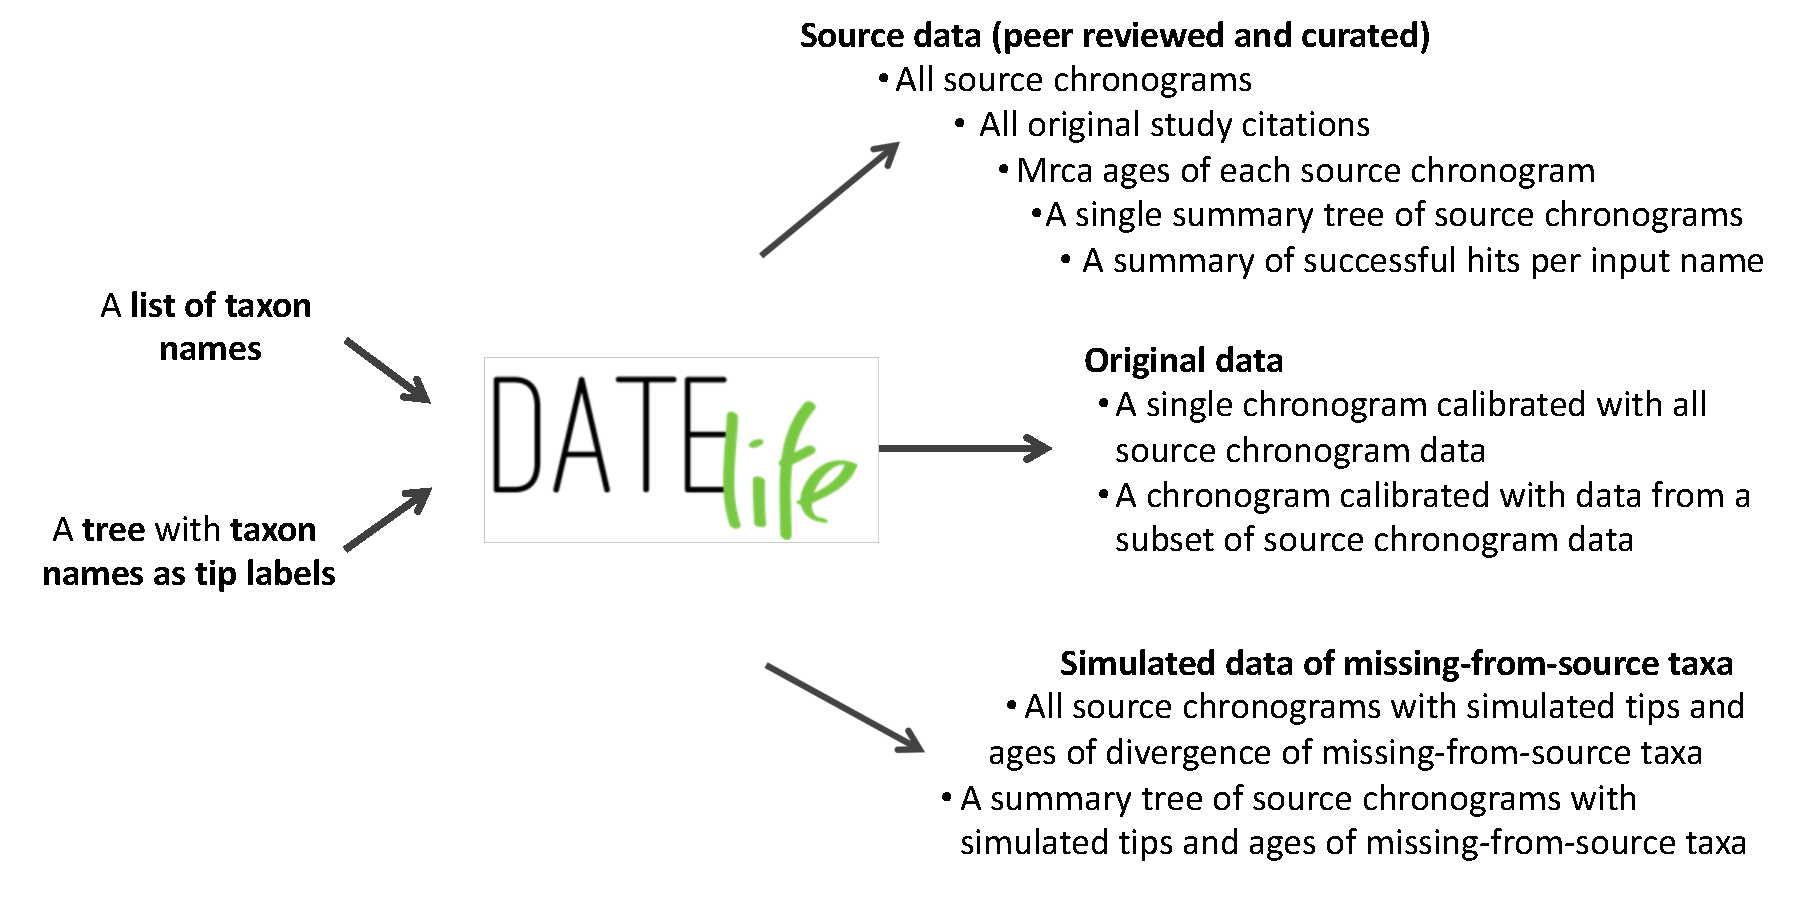
\includegraphics{../figures/Fig1.pdf}
\caption{Stylized DateLife workflow. This shows the general workflows and analyses that can be performed with \texttt{datelife}, via the R package or through the website  at \url{www.datelife.org/query/}. Details on the functions involved on each workflow are shown in \texttt{datelife}'s R package vignette.}
\label{fig:workflow}
\end{figure}
% \begin{center}
% \textsc{Figure \ref{fig:workflow}}
% \end{center}
% Stylized DateLife workflow. This shows the general workflows and analyses that can be performed with \texttt{datelife}, via the R package or through the website  at \url{http://www.datelife.org/}. Details on the functions involved on each workflow are shown in \texttt{datelife}'s R package vignette.
\newpage
\begin{figure}[!h]
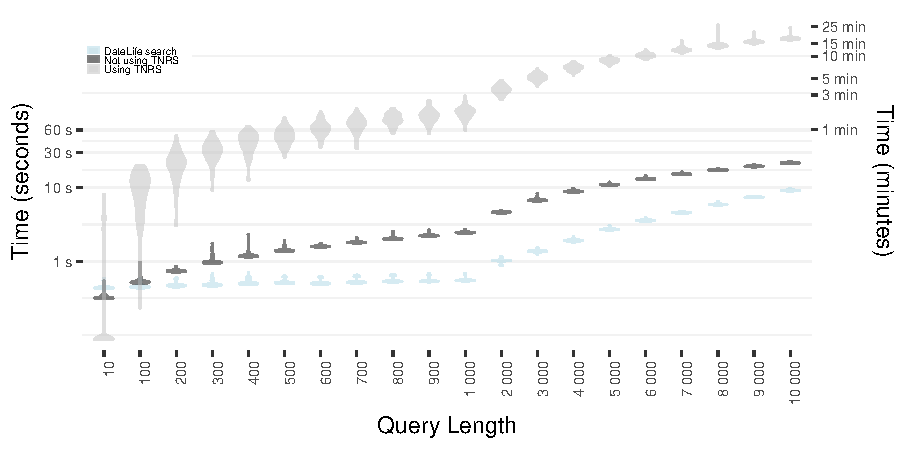
\includegraphics[width=1\linewidth]{../figures/fig_runtime_main.pdf}
\caption{Input taxon name processing and chronogram database search computation time increases with number of input taxon names. We sampled N bird species names for each input size class, 100 times, and then performed a \texttt{datelife} search using the Taxon Names Resoultion Service (TNRS; dark gray), and without using TNRS (light gray). We also performed a search using the already processed query for comparison (light blue).}
\label{fig:runtime1}
\end{figure}
% \begin{center}
% \textsc{Figure \ref{fig:runtime1}}
% \end{center}
% 
\newpage
\begin{figure}[!h]
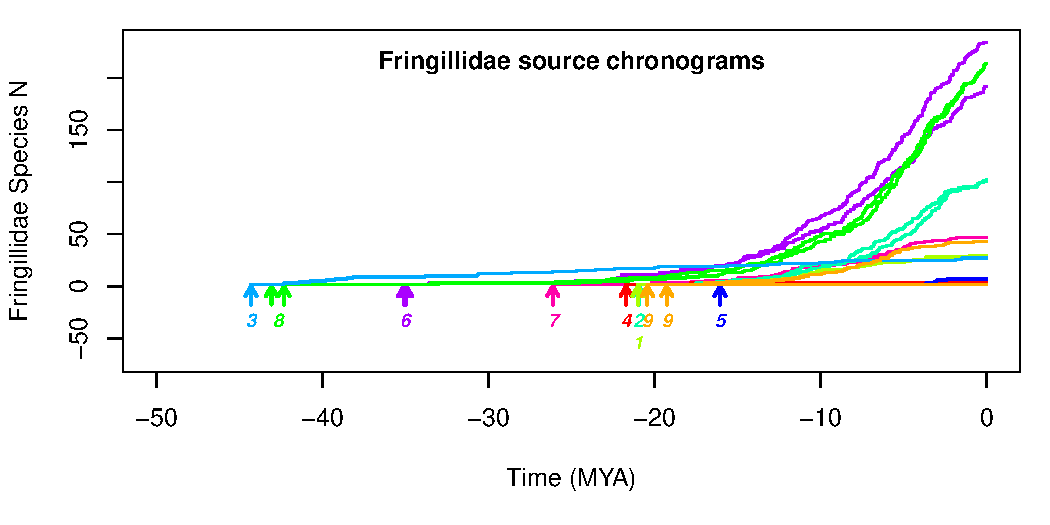
\includegraphics[width=1\linewidth]{../figures/fig_schronograms1.pdf}
\caption{Lineage through time (LTT) plots of source chronograms containing all or a subset of species from the bird family Fringillidae of true finches. Arrows indicate maximum age of each chronogram. Numbers reference to chronograms' original publications 1: Barker et al. (\protect\hyperlink{ref-barker2012going}{2012}), 2: Barker et al. (\protect\hyperlink{ref-barker2015new}{2015}), 3: Burns et al. (\protect\hyperlink{ref-burns2014phylogenetics}{2014}), 4: Claramunt and Cracraft (\protect\hyperlink{ref-claramunt2015new}{2015}), 5: Gibb et al. (\protect\hyperlink{ref-gibb2015new}{2015}), 6: Hedges et al. (\protect\hyperlink{ref-Hedges2015}{2015}), 7: Hooper and Price (\protect\hyperlink{ref-hooper2017chromosomal}{2017}), 8: Jetz et al. (\protect\hyperlink{ref-Jetz2012}{2012}), 9: Price et al. (\protect\hyperlink{ref-price2014niche}{2014}).
}
\label{fig:schronograms1}
\end{figure}
% \begin{center}
% \textsc{Figure \ref{fig:schronograms1}}
% \end{center}
%Lineage through time (LTT) plots of source chronograms containing all or a subset of species from the bird family Fringillidae of true finches. Arrows indicate maximum age of each chronogram. Numbers reference to chronograms' original publications 1: Barker et al. (\protect\hyperlink{ref-barker2012going}{2012}), 2: Barker et al. (\protect\hyperlink{ref-barker2015new}{2015}), 3: Burns et al. (\protect\hyperlink{ref-burns2014phylogenetics}{2014}), 4: Claramunt and Cracraft (\protect\hyperlink{ref-claramunt2015new}{2015}), 5: Gibb et al. (\protect\hyperlink{ref-gibb2015new}{2015}), 6: Hedges et al. (\protect\hyperlink{ref-Hedges2015}{2015}), 7: Hooper and Price (\protect\hyperlink{ref-hooper2017chromosomal}{2017}), 8: Jetz et al. (\protect\hyperlink{ref-Jetz2012}{2012}), 9: Price et al. (\protect\hyperlink{ref-price2014niche}{2014}).
\newpage
\begin{figure}[!h]
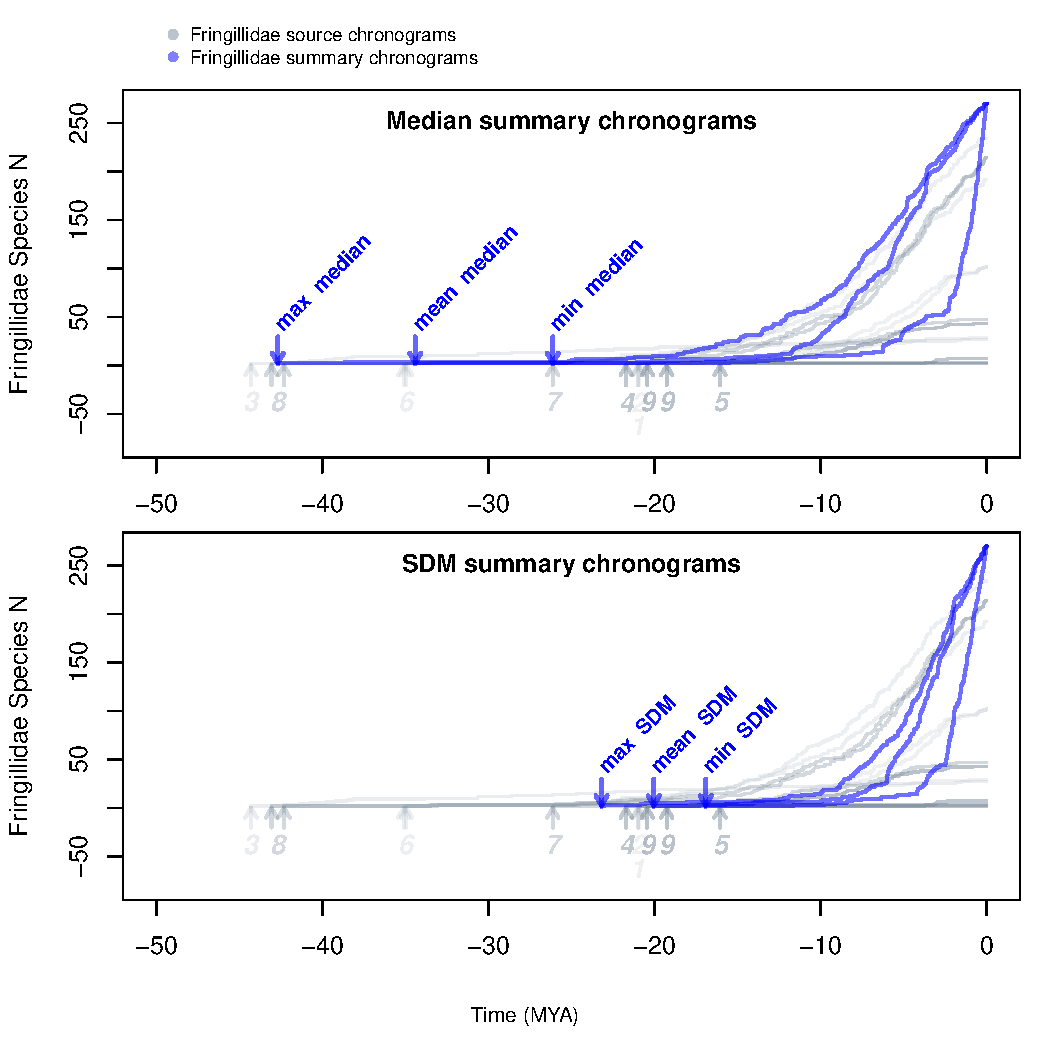
\includegraphics{../figures/fig_summaries.pdf}
\caption{LTT plots of median (top) and Supermatrix Distance Method (SDM; bottom) chronograms summarising information from source chronograms found for the Fringillidae. Arrows indicate tree maximum age.}
\label{fig:summaries}
\end{figure}
% \begin{center}
% \textsc{Figure \ref{fig:summaries}}
% \end{center}
% LTT plots of median (top) and Supermatrix Distance Method (SDM; bottom) chronograms summarising information from source chronograms found for the Fringillidae. Arrows indicate tree maximum age.
\newpage
\begin{figure}[!h]
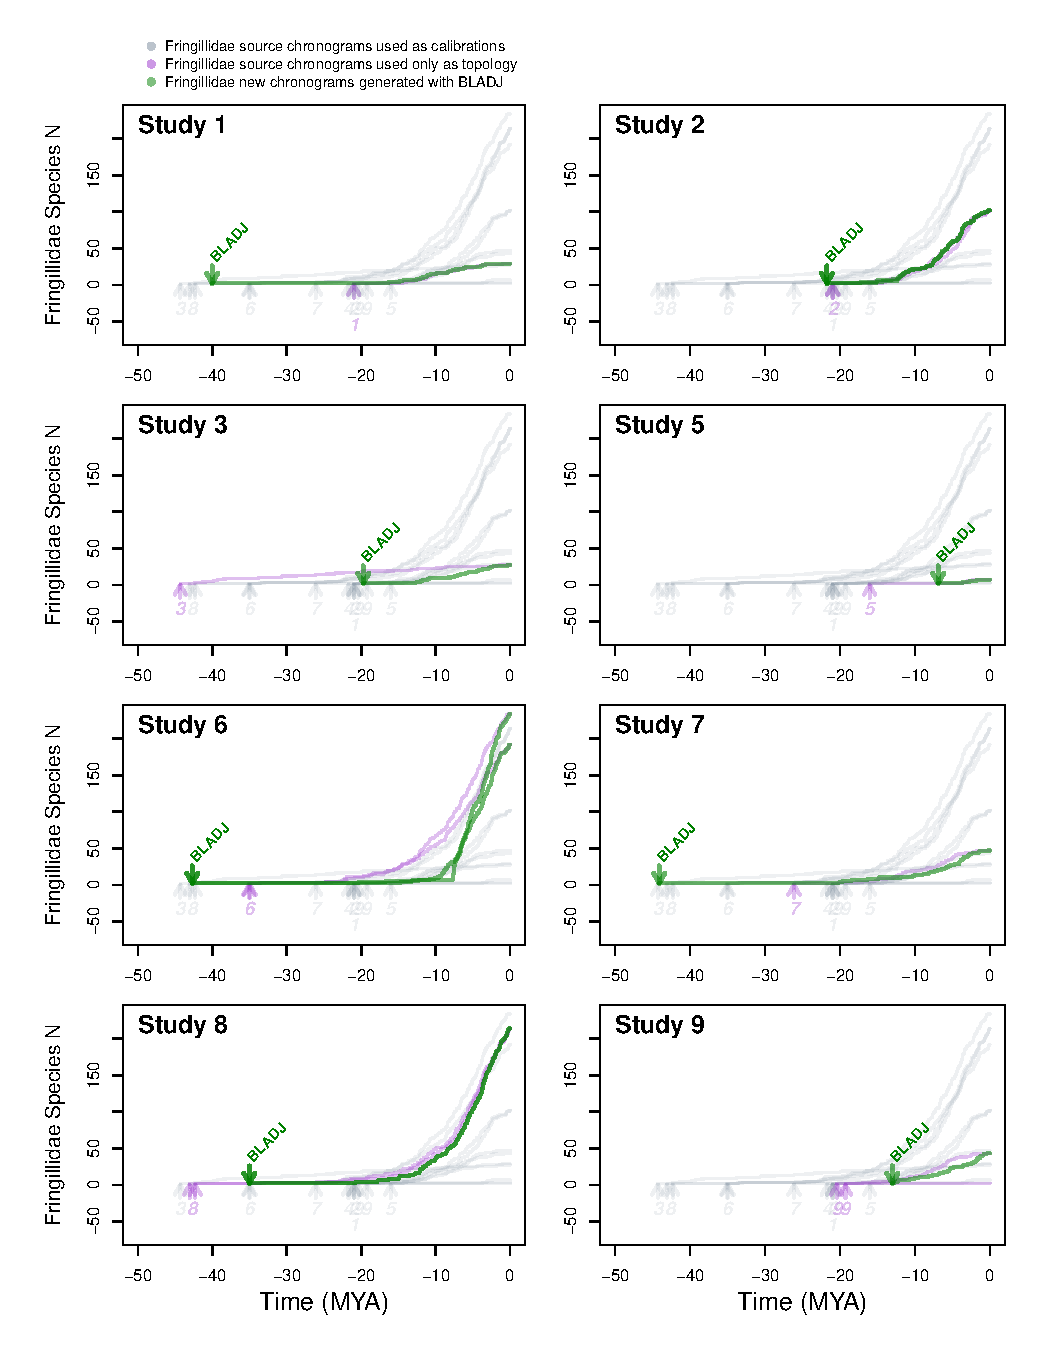
\includegraphics{../figures/fig_crossval_bladj.pdf}
\caption{LTT plots showing results from the cross-validation analyses of trees without branch lengths dated using BLADJ. The dating analysis can only be performed in trees with more than 2 tips, thus excluding chronogram from study 4; its data was still used as calibration for the other source chronograms.}
\label{fig:cvbladj}
\end{figure}
% \begin{center}
% \textsc{Figure \ref{fig:cvbladj}}
% \end{center}
% LTT plots showing results from the cross-validation analyses of trees without branch lengths dated using BLADJ. The dating analysis can only be performed in trees with more than 2 tips, thus excluding chronogram from study 4; its data was still used as calibration for the other source chronograms.
\newpage
\begin{figure}[!h]
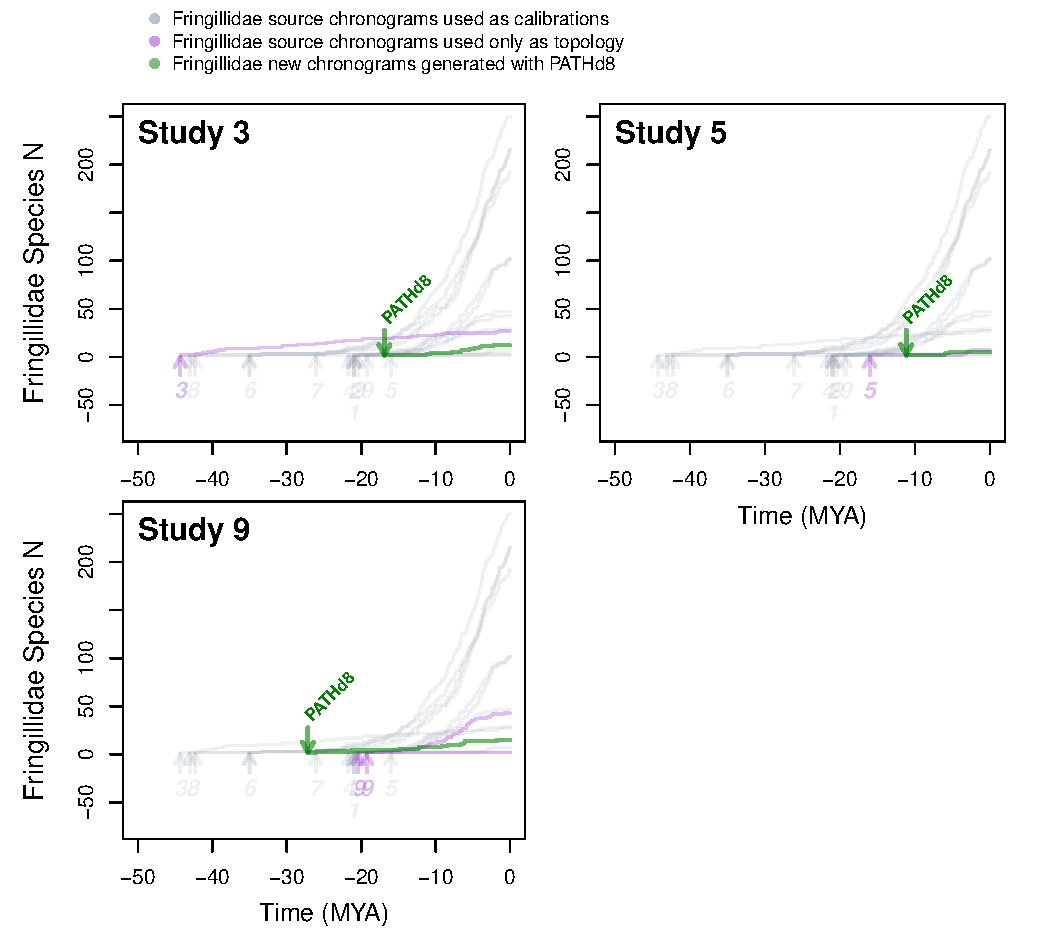
\includegraphics{../figures/fig_crossval_boldsumm.pdf}
\caption{LTT plots showing results from the cross-validation analyses of trees with branch length reconstructed with data from the Barcode of Life Database (BOLD) dated using PATHd8. We could construct a tree with branch lengths for all source chronograms. However, dating with PATHd8 was only successful in three source chronograms shown here.}
\label{fig:cvbold}
\end{figure}
% \begin{center}
% \textsc{Figure \ref{fig:cvbold}}
% \end{center}
FIGURES
%LTT plots showing results from the cross-validation analyses of trees with branch length reconstructed with data from the Barcode of Life Database (BOLD) dated using PATHd8. We could construct a tree with branch lengths for all source chronograms. However, dating with PATHd8 was only successful in three source chronograms shown here.

%\end{linenumbers}

\end{document}
